
\documentclass[%
pdftex,
oneside,			% Einseitiger Druck.
11pt,				% Schriftgroesse
parskip=half,		% Halbe Zeile Abstand zwischen Absätzen.
%	topmargin = 10pt,	% Abstand Seitenrand (Std:1in) zu Kopfzeile [laut log: unused]
headheight = 12pt,	% Höhe der Kopfzeile
%	headsep = 30pt,	% Abstand zwischen Kopfzeile und Text Body  [laut log: unused]
headsepline,		% Linie nach Kopfzeile.
footsepline,		% Linie vor Fusszeile.
footheight = 16pt,	% Höhe der Fusszeile
abstracton,		% Abstract Überschriften
DIV=calc,		% Satzspiegel berechnen
BCOR=8mm,		% Bindekorrektur links: 8mm
headinclude=false,	% Kopfzeile nicht in den Satzspiegel einbeziehen
footinclude=false,	% Fußzeile nicht in den Satzspiegel einbeziehen
listof=totoc,		% Abbildungs-/ Tabellenverzeichnis im Inhaltsverzeichnis darstellen
toc=bibliography,	% Literaturverzeichnis im Inhaltsverzeichnis darstellen
]{scrreprt}	% Koma-Script report-Klasse, fuer laengere Bachelorarbeiten alternativ auch: scrbook


\def \titel {Konzeption -- Entwicklung eines real-time Backends für eine datenintensive Applikation}
\def \arbeit {Seminararbeit}
\def \autor {Jasper Bremenkamp}
\def \abschluss {Master of Science}
\def \studiengang {Data Science}
\def \datumAbgabe {\today}
\def \modul {Projekt: Data Engineering}
\def \matrikelnr {92125193}
\def \tutor {Prof. Dr. Max Pumperla}

\def \seitenrand {2cm}

% PDF Einstellungen
\usepackage{hyperref}

\hypersetup{
    unicode = true,
    pdftitle={\titel},
    pdfauthor={\autor},
    pdfsubject={\arbeit},
    pdfcreator={pdflatex, LaTeX with KOMA-Script},
    pdfpagemode=UseOutlines, 		% Beim Oeffnen Inhaltsverzeichnis anzeigen
    pdfdisplaydoctitle=true, 		% Dokumenttitel statt Dateiname anzeigen.
    pdflang={de}, 			% Sprache des Dokuments.
    hidelinks
}

\usepackage[left=2cm,right=2cm,top=2cm,bottom=2cm]{geometry} % margins	% Seitenränder und Abstände
\usepackage[activate]{microtype} %Zeilenumbruch und mehr
\usepackage[onehalfspacing]{setspace}
\usepackage{makeidx}
\usepackage[autostyle=true,german=quotes]{csquotes}
\MakeOuterQuote{"} % Für deutsche Anführungszeichen
\usepackage{longtable}
\usepackage{enumitem}	% mehr Optionen bei Aufzählungen
\usepackage{graphicx}
\usepackage{pdfpages}   % zum Einbinden von PDFs
\usepackage{xcolor} 	% für HTML-Notation
\usepackage{float}
\usepackage{array}
\usepackage{calc}		% zum Rechnen (Bildtabelle in Deckblatt)
\usepackage[right]{eurosym}
\usepackage{wrapfig}
\usepackage{pgffor} % für automatische Kapiteldateieinbindung
\usepackage[perpage, hang, multiple, stable]{footmisc} % Fussnoten
\usepackage[printonlyused]{acronym} % falls gewünscht kann die Option footnote eingefügt werden, dann wird die Erklärung nicht inline sondern in einer Fußnote dargestellt
\usepackage{listings}
\usepackage{bookmark}
\usepackage[english, ngerman]{babel}
\usepackage[utf8]{inputenc}
\usepackage{scrhack}
\usepackage{txfonts} % Use a Times-new-roman open-source clone


    %%%%%%% Neues Design %%%%%%%%%%%
    \setkomafont{chapter}{\Large}
    \setkomafont{section}{\large}
    \setkomafont{subsection}{\large}

    %\renewcommand*\chapterheadstartvskip{\vspace*{-0cm}} %Kapitel nach oben verschieben

    \addtolength{\footskip}{-0.7cm}% foot larger by 0,7 cm  (Raises the page number)
    \setlength{\parindent}{6pt} % Indent at start of paragraphs  6pt

    \renewcommand\thesection{\arabic{section}}
    \renewcommand\thefigure{\arabic{figure}}

    %%%%%%%%%%%%%%%%%%%%%%%%%%%%%%%

% Notizen. Einsatz mit \todo{Notiz} oder \todo[inline]{Notiz}.
\usepackage[obeyFinal,backgroundcolor=yellow,linecolor=black]{todonotes}
% Alle Notizen ausblenden mit der Option "final" in \documentclass[...] oder durch das auskommentieren folgender Zeile
% \usepackage[disable]{todonotes}

% Kommentarumgebung. Einsatz mit \comment{}. Alle Kommentare ausblenden mit dem Auskommentieren der folgenden und dem aktivieren der nächsten Zeile.
\newcommand{\comment}[1]{\par {\bfseries \color{blue} #1 \par}} %Kommentar anzeigen

% der neue Zitierstil ist Käse
\global\def\VAlterZitierstil{true}

\global\def\VTrueValue{true}

\ifx\VAlterZitierstil\VTrueValue
    \usepackage[
        backend=bibtex,     % empfohlen. Falls biber Probleme macht: bibtex
        bibwarn=true,
        bibencoding=utf8,   % wenn .bib in utf8, sonst ascii
        sortlocale=de_DE,
        sorting=none,
        style=numeric-comp
    ]{biblatex}

    \addbibresource{bibliographie.bib}
\else
    % New IUBH Cite Style / Old Cite style below
    \usepackage{natbib}
    \setcitestyle{aysep={}} % remove comma as delimiter
\fi


\begin{document}

\pagenumbering{Roman}

\begin{titlepage}
    \pdfbookmark{\titel}{}
    \begin{longtable}{p{7cm} p{12cm}}
        {\raisebox{\ht\strutbox-\totalheight}{
\includegraphics[height=3cm]{assets/iu.png}}}
    \end{longtable}
    \enlargethispage{20mm}
    \begin{center}
        \vspace*{12mm}	{\LARGE\textbf \titel }\\
        \vspace*{12mm}	{\large\textbf \arbeit}\\
        \vspace*{12mm}	Prüfungsleistung für den\\
        \vspace*{3mm}		{\textbf \abschluss}\\
        \vspace*{12mm}	des Studiengangs \studiengang\\
    \vspace*{3mm}		an der Internationalen Hochschule\\
        \vspace*{12mm}	von\\
        \vspace*{3mm}		{\large\textbf \autor}\\
        \vspace*{12mm}	\datumAbgabe
    \end{center}
    \vfill
    \begin{spacing}{1.2}
    \begin{tabbing}
        mmmmmmmmmmmmmmmmmmmmmmmmmm             \= \kill
        \textbf{Kursbezeichnung} \> \modul\\
        \textbf{Matrikelnummer} \> \matrikelnr\\
        \textbf{Tutor} \> \tutor\\
    \end{tabbing}
    \end{spacing}
\end{titlepage}

\newpage

%Abbildungsverzeichnis
%\cleardoublepage %To-Do: Wieder hinzufügen, wenn sinnvolle Grafiken eingefügt werden
%\listoffigures

%Tabellenverzeichnis
%\cleardoublepage
%\listoftables

%\chapter{Konzeption} %evtl weg lassen und section sind dann chapter
\pagenumbering{arabic}

% \comment{Inhalt: \\
% Beschreibung des Hintergrund-Szenarios \\
% Dokumentierung von Informationslücken \\
% Strategie zur Beschaffung/Füllung der Informationslücken \\
% }

% \comment{Anforderungen: \\
% Nicht mehr als 2 Seiten
% Diagramme und Schaubilder nach Ermessen einsetzbar
% }

\section{Szenario}

    Die Frischmarkt AG, eine Kette von Lebensmittelgeschäften, steht vor der Aufgabe, datengestützte Entscheidungsfindung in ihre Betriebsprozesse zu integrieren, um Effizienz zu steigern, Kosten zu senken und die Kundenzufriedenheit zu verbessern.
    Die derzeitige Infrastruktur, bestehend aus Kassensystemen, Lagerverwaltung und Kundendatenbanken, wird hauptsächlich zur Datenspeicherung genutzt, jedoch nicht für fortschrittliche Analysen oder Echtzeit-Entscheidungen.

    Das Ziel des Projekts ist der Aufbau einer Dateninfrastruktur, die in der Lage ist, kontinuierlich große Mengen an Echtzeitdaten zu verarbeiten und automatisierte Prozesse zu ermöglichen.
    Ein Schwerpunkt liegt auf der automatisierten Bestandsverwaltung, dynamischen Preisgestaltung und personalisierten Angeboten.
    Automatisierte Nachbestellungen sollen auf Grundlage von Verkaufsdaten, Lagerbeständen und saisonalen Schwankungen ausgelöst werden.

\section{Strategie}

    Um diese Ziele zu erreichen, verfolgt die Frischmarkt AG eine mehrstufige Strategie zur Entwicklung einer effizienten Datenverarbeitungsarchitektur.

    %\subsection{Modulare und skalierbare Architektur}

    Ein zentrales Prinzip der Strategie ist der Aufbau einer modularen und skalierbaren Architektur auf Basis einer Microservice-Architektur.
    Kubernetes und Helm werden als Werkzeuge für Infrastructure as Code (IaC) verwendet, um die Skalierbarkeit und Wartbarkeit des Systems zu gewährleisten.
    Kubernetes orchestriert die Microservices, um ihre Skalierung und Fehlertoleranz zu gewährleisten.

    Für die Containerisierung wird Podman anstelle der mehr bekannten Docker Container Engine verwendet, da Podman keinerlei proprietäre Einschränkungen wie Docker hat und außerdem einige Vorteile gegenüber Docker bietet, wie z. B. Rootless Containers, welche die Sicherheit erhöhen.
    Podman kann problemlos im Zusammenhang mit Kubernetes-Umgebungen genutzt werden und unterstützt ebenfalls die wesentlichen Features, die Docker bietet.

    Die Architektur teilt das System in unabhängige Komponenten auf, z.B. Datenaufnahme und -verarbeitung, die von Apache Kafka als Nachrichten-Streaming-Plattform übernommen wird.
    Diese Modularität erleichtert die Skalierbarkeit des Systems, da einzelne Services unabhängig skaliert oder aktualisiert werden können.

    %\subsection{Schrittweise Einführung und Testing}
    %Die Implementierung erfolgt in mehreren Phasen, um Risiken zu minimieren und eine kontinuierliche Verbesserung zu ermöglichen:

    %\begin{itemize}
    %    \item \textbf{Phase 1: Konzeptionsphase} – In dieser Phase wird eine gründliche Analyse der bestehenden Systeme und der erforderlichen Technologien durchgeführt.
    %    Neben der Auswahl von Apache Kafka für die Datenaufnahme und das Streaming wird die Infrastruktur mithilfe von Kubernetes und Helm definiert.
    %    GitHub wird für die Versionskontrolle genutzt, um Nachvollziehbarkeit und Reproduzierbarkeit sicherzustellen.
    %
    %    \item \textbf{Phase 2: Implementierung und Integration} – Die eigentliche Entwicklung der Microservices beginnt, inklusive der Integration von Kassensystemen und Lagerverwaltung.
    %    Da in dieser Phase noch kein Zugang zu den produktiven Systemen besteht, werden Mocks oder Fakes verwendet, die als simulierte Datenquellen dienen.
    %    Diese Fakes publizieren simulierte Daten an Kafka Topics, um die Datenpipeline zu testen.
    %
    %    \item \textbf{Phase 3: Skalierung und Optimierung} – In dieser Phase wird das System auf größere Datenmengen skaliert und in den produktiven Betrieb überführt.
    %    Dabei wird der Fokus auf die Optimierung der Datenströme und der Algorithmen gelegt, um Echtzeit-Entscheidungen und Vorhersagen zu verbessern.
    %\end{itemize}

    %\subsection{Automatisierte Bestandsverwaltung}

    % Die automatisierte Bestandsverwaltung ist ein Kernziel des Projekts und wird in diesem Abschnitt beschrieben.
    Ein zentraler Aspekt des Systems ist die automatisierte Bestands- und Verkaufserfassung.
    Verkaufs- und Lagerbestandsdaten werden kontinuierlich über Apache Kafka gesammelt und in Echtzeit verarbeitet.

    Das Sammeln der Daten wird in den Filialen oder anderen Einrichtungen des Unternehmens von unabhängigen kleinen Rechnern übernommen, um möglichst flexibel mit den Gegebenheiten vor Ort umgehen zu können.
    Ohne zusätzlichen Computer ist das direkte Senden der Daten aus der Kasse direkt zu Kafka technisch schwer realisierbar, da es keine einfache Möglichkeit gibt containerisierte Microservices darauf auszuführen.
    Daher werden die Microservices auf seperaten Rechnern ausgeführt und es werden die Schnittstellen zu den Systemen vor Ort, wie u. a. die Kassensysteme genutzt.
    So lassen sich für unterschiedliche Betriebsstätten auch verschiedene Microservices einsetzen, die ihre vorberarbeiteten Daten an eine zentrale Stelle senden.
    Da die Datenvorprozessierung und Aggregation bereits außerhalb des eigentlichen Rechenzentrums stattfindet handelt es sich bei dem Konzept u. a. auch um Edge Computing.

    Während der Entwicklungsphase werden Fakes verwendet, welche diese Rechner dann nachstellen, um Datenströme zu simulieren und die automatisierte Bestandsverwaltung zu testen, bevor das System mit realen Daten verknüpft wird.
    Die zusendenden Daten sollen auf eine Minute zusammengefasst sein.
    Die Einführung dieser Verwaltung würde nach Abschluss schrittweise in Pilotfilialen erfolgen, um die Effizienz und Anpassungsfähigkeit an regionale und saisonale Unterschiede zu testen.
    Kubernetes ermöglicht die flexible Skalierung der Infrastruktur, um die Datenanforderungen zu bewältigen.
    Im Rahmen der Entwicklung wird das Kernsystem nur auf ein Single-Node Cluster ausgerollt und die Edge-Computer Microservices in einem eigenen Namespace.
    Später im Produktivbetrieb lässt sich dann ohne zusätzlichen Aufwand auf ein Multi-Node Cluster oder ein High Availability (HA) Cluster bestehend aus mehreren anderen Clustern umsteigen und die Edge-Computer Microservices lassen sich auf kleinere Rechner vor Ort ausrollen.

    %\subsection{Datenbasierte Entscheidungsfindung}

    Die datengestützte Entscheidungsfindung wird durch Echtzeit-Datenanalysen ermöglicht, die es dem Management erlauben, auf aktuelle Entwicklungen in den Filialen zu reagieren.
    Mithilfe von Machine Learning-Algorithmen werden Verkaufsprognosen erstellt, die u. a. dynamische Preisanpassungen und personalisierte Angebote unterstützen.
    Diese Algorithmen werden kontinuierlich mit aktuellen Verkaufs- und Lagerdaten sowie weiteren relevanten Daten trainiert, die über Kafka in das System eingespeist werden.
    In der Entwicklungsphase wird dies mit simulierten Daten getestet.

    Obwohl Machine Learning eine zentrale Rolle in der zukünftigen Entwicklung spielt, liegt der Fokus dieses Projekts auf der Implementierung der zugrunde liegenden Dateninfrastruktur.
    Die konkrete Implementierung der Machine Learning Algorithmen wird nicht abgehandelt.

    %\subsection{Integration und Datenquellen}

    Die nahtlose Integration bestehender Systeme ist ein weiterer strategischer Fokus.
    Die Kassensysteme und CRM-Systeme der Frischmarkt AG sollen in die neue Dateninfrastruktur eingebunden werden, wobei Apache Kafka als zentrale Plattform für die Datenaufnahme fungiert.

    Da der Zugang zu produktiven Datenquellen in der Entwicklungsphase noch nicht gegeben ist, werden wie bereits erläutert Fakes verwendet, um Kassendaten, Lagerbestände und andere Daten zu simulieren.
    Diese Fakes publizieren vorprozessierte Daten an Kafka Topics, um den realen Betrieb zu simulieren und die Datenpipeline unter realistischen Bedingungen zu testen.
    Die Fakes übernehmen damit auch die Aufgabe der Vorprozessierung, die im Produktivbetrieb von dem Edge-Computer und dessen Microservice(s) gemacht werden würden.
    Anschließend werden die publizierten Daten aus den Topics von verschiedenen Microservices konsumiert und für die verschiedenen Anwendungsfälle verarbeitet und anschließend in den Datensenken bereitgestellt.

    Die Ziel-Architektur ist in nachfolgender Abbildung \ref{fig:architekturentwurf} vereinfacht dargestellt.

    \begin{figure}[H]
        \centering
        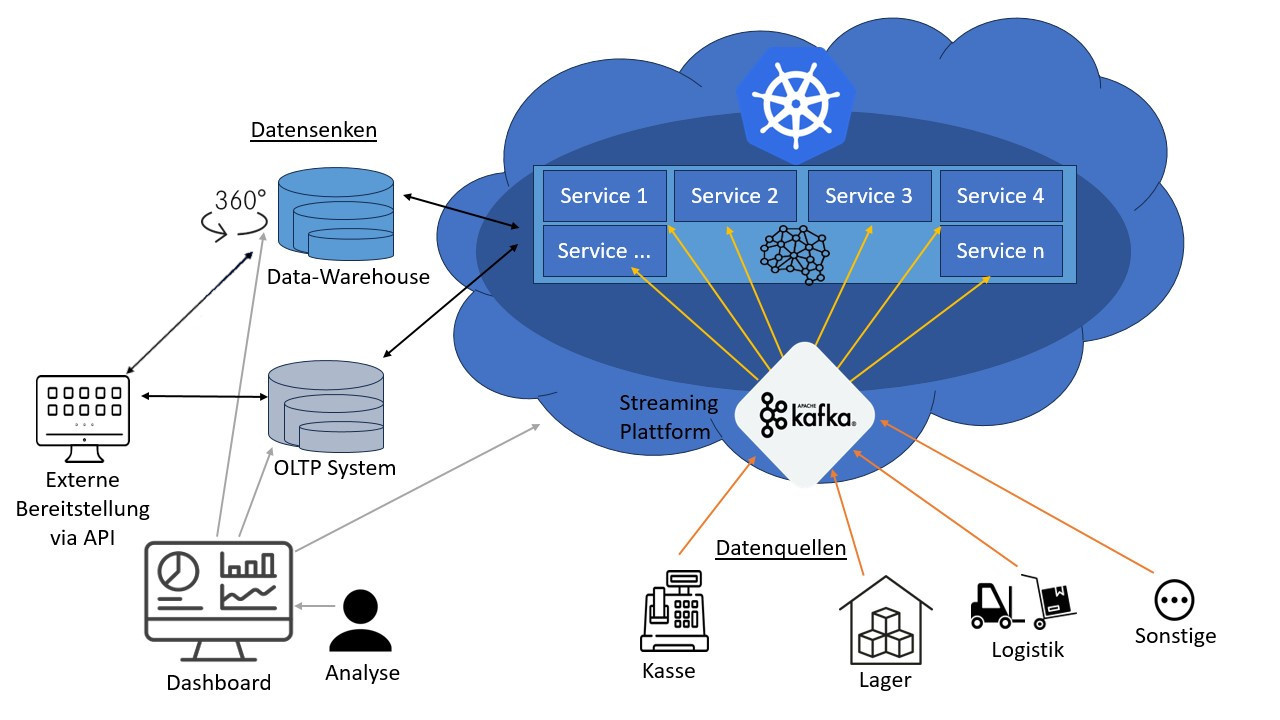
\includegraphics[width=1\textwidth]{assets/architekturentwurf.jpg}
        \caption{Architekturübersicht}
        \label{fig:architekturentwurf}
    \end{figure}

    Die Exklusion der API und der Datensenken aus dem Kubernetes Cluster in der Abbildung \ref{fig:architekturentwurf} ist lediglich implizit.
    Das bedeutet, dass sie nicht unbedingt im Kubernetes-Cluster betrieben werden müssen, da sie keine unbedingt skalierbaren Microservices darstellen.
    Im Rahmen der Entwicklung werden sie jedoch ebenfalls im Cluster bereitgestellt.

    Apache Kafka und andere Softwarebestandteile, die keine Eigenentwicklung sind, werden über Helm Packages installiert.
    Darin sind ebenfalls auch die \enquote{richtigen Docker-Images} hinterlegt.
    Ein gut geeigntes Helm Package für Kafka ist z. B. folgendes: \url{https://artifacthub.io/packages/helm/bitnami/kafka}.

    Die Entscheidung für diese Microservice-Architektur bietet mehrere wesentliche Vorteile:
    \begin{itemize}
        \item \textbf{Skalierbarkeit durch Microservices}: Die Nutzung von Kubernetes ermöglicht eine flexible und effiziente Skalierung der einzelnen Services.
        \item \textbf{Flexibilität durch Kafka}: Kafka entkoppelt Datenquellen und -senken, was eine flexible Integration neuer Datenquellen ermöglicht.
        \item \textbf{Echtzeit-Datenverarbeitung}: Kafka bietet nahezu sofortige Datenweitergabe, was in Echtzeit Entscheidungen ermöglicht.
        \item \textbf{Zentralisierte Datenverarbeitung}: OLTP-Systeme und Data-Warehouses ermöglichen parallele Nutzung für operative und analytische Zwecke.
        \item \textbf{Modularität und Wartbarkeit}: Jeder Dienst kann unabhängig entwickelt und gewartet werden, was die Agilität erhöht.
    \end{itemize}

    Es gibt jedoch auch einige Nachteile, die mit dieser Architektur verbunden sind:
    \begin{itemize}
        \item \textbf{Komplexität der Integration}: Die Integration von Kafka, Kubernetes und Microservices erfordert erhebliche technische Expertise.
        \item \textbf{Erhöhter Wartungsaufwand}: Die verteilte Architektur erfordert eine kontinuierliche Überwachung und Pflege.
        \item \textbf{Datenkonsistenz}: In einer verteilten, asynchronen Umgebung besteht ein Risiko für inkonsistente Daten zwischen verschiedenen Systemen.
    \end{itemize}

    %\subsection{Datensicherheit und Datenschutz}

    Datensicherheit und Datenschutz sind ebenfalls zentrale Bestandteile.
    Erfasste Kundendaten werden gemäß der Datenschutz-Grundverordnung (DSGVO) verarbeitet.
    Die Speicherung und Verarbeitung der Daten erfolgt verschlüsselt, und es werden strenge Zugangskontrollen implementiert.

    Um die Einhaltung der Datenschutzanforderungen sicherzustellen, werden Sicherheitsmechanismen wie verschlüsselte Datenübertragungen und in Zukunft regelmäßige Sicherheitsaudits in die Infrastruktur integriert.
    Ein Data Governance-Framework regelt den Umgang mit den Daten und gewährleistet Transparenz.

    %\subsection{Zusammenarbeit und Versionskontrolle}

    Die Zusammenarbeit zwischen den internen IT-Teams der Frischmarkt AG und externen Experten ist entscheidend für den Erfolg des Projekts.
    Git in Verbindung mit GitHub als Plattform wird für die Versionskontrolle genutzt, um eine klare Rückverfolgbarkeit der Änderungen und eine kollaborative Entwicklung in verteilten Teams zu ermöglichen.

    %\subsection{Schlussfolgerung}

    Die Strategie zur Entwicklung der Dateninfrastruktur für die Frischmarkt AG basiert auf einer modularen, skalierbaren Architektur, die Kubernetes, Helm und Podman verwendet, um die Skalierbarkeit, Wartbarkeit und Verfügbarkeit des Systems sicherzustellen.
    Apache Kafka wird als zentrale Plattform für die Datenaufnahme und -verarbeitung eingesetzt.
    Simulierte Datenquellen werden genutzt, um die Datenpipeline während der Entwicklungsphase zu testen.
    Datensicherheit und Datenschutz haben höchste Priorität, um den gesetzlichen Anforderungen gerecht zu werden.


% To-Dos:
% Inhalt eindampfen
% Prüfen wie lang der Inhalt der Konzeption in diesem Modul sein darf
% Falls länger, dann ein Kapitel zur technischen Details einbauen und auf Helm templates, Images und die anderen Fragen unter diesem Satz eingehen.


%Folgende Fragen klären:
% Am Ende dieser Phase fertigst Du eine konzeptionelle Zeichnung Deiner Dateninfrastruktur an. Außerdem solltest Du dabei für Dich selbst folgende Fragen beantworten können:
% • Welcher Microservice wird data ingestion in mein System übernehmen?                                                                             Die an der Kante
% • Welcher Microservice wird die Datenvorprozessierung und Aggregation übernehmen?                                                                 Die an der Kante
% • Mit welchen Techniken und Methoden stelle ich sicher, dass mein System zuverlässig (reliable), skalierbar (scalable) und wartbar (maintainable) ist? Kubernetes & Helm
% • Mit welchen Techniken stelle ich sicher, dass Datenschutz, Datensicherheit und Data Governance in meinem System berücksichtigt werden?          Data Governance-Framework
% • Welche Docker Images werde ich nutzen, um mein System aufzubauen und müssen diese gegebenenfalls modifiziert werden?                            Die aus Helm
% • Welche Daten werde ich verwenden, um mein System zu testen?                                                                                     Fake-Daten
% • Welche Aggregations- und Windowing-Funktionen werde ich nutzen, um die Daten zu aggregieren?

% Abschließend stellst Du Deine Gedanken und Recherchen in einer konzeptionellen Flow-Chart-Zeichnung zum
% Entwurf Deiner Architektur zusammen. Zur Inspiration kannst Du beispielsweise die Referenzarchitekturen der
% großen Cloud Provider nutzen (bspw. Microsoft Azure Reference Architecture: https://docs.microsoft.com/en-gb/azure/architecture/browse/ [letzter Zugriff: 11.11.2020]). Außerdem solltest Du die Vor- und Nachteile Deiner
% konzeptionellen Architektur diskutieren.


\ifx\VAlterZitierstil\VTrueValue
    \printbibliography
\else
    \bibliographystyle{iubh}
    \bibliography{bibliographie.bib}
\fi
\end{document}
